\usetikzlibrary{arrows.meta}
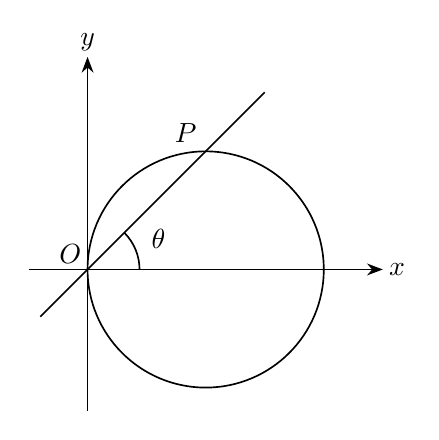
\begin{tikzpicture}[x=3cm,y=3cm,line width=.6pt,>=Stealth,font=\normalsize]
\coordinate (O) at (0,0);
\coordinate (P) at (0.5,0.5);
\draw[->] (-0.25,0)--(1.25,0) node[right,inner sep=2pt] {$x$};
\draw[->] (0,-0.6)--(0,0.9) node[above,inner sep=2pt] {$y$};
\draw (0.5,0) circle [radius=0.5];
\draw (-0.2,-0.2)--(0.75,0.75);
\draw (0.22,0) arc[start angle=0,end angle=45,radius=0.22];
\node[above left,inner sep=2pt] at (O) {$O$};
\node[above left,inner sep=3pt] at (P) {$P$};
\node at (0.3,0.13) {$\theta$};
\end{tikzpicture}
